\chapter{Бекаа-82. Часть 2. Судный день сирийских ПВО}
\begin{remark}
	"... Под нами ад. Всё, что может, стреляет в воздух. Ощущение, как будто земля поднялась на несколько километров вверх. Да, для того, чтобы атаковать, придётся нырять во всё это.
	
	Как по команде (а так оно и есть), по часовой стрелке вспыхивают маленькие шарики в дулах орудий, направленных на меня.
	
	Краем глаза слежу за стрелками скорости и высоты, и вот стрелка высоты подходит к отметке, в унисон ей довожу мушку прицела к центру батареи. А там, в центре мозг батареи, из него к каждому орудию идут кабели с данными по наводке на цель, то есть на меня.
	
	Я нажимаю на кнопку бомбометания и чувствую удар под брюхом: мой подарок командиру батареи весом в тонну поехал по своей баллистической траектории. Тяну на себя ручку управления и перехожу из пике в набор высоты в развороте.... "
\end{remark}

«Арцав-19», знаменитая операция израильтян в долине Бекаа 9 июня вошла в историю воздушных войн. Менее чем за сутки 15 из 19 сирийских дивизионов ЗРК были уничтожены. Попытка спасти их силами авиации стоила сирийцам 30 самолётов. Управление операцией осуществлялось практически «в прямом эфире» — впервые в мире. И — без потерь. Как это было?

Первая Ливанская война началась 6 июня 1982 года. Поводом для вторжения израильтян в Ливан стало покушение на посла этой страны в Лондоне Шломо Аргова (он выжил, но остался инвалидом). После этого израильские лидеры решили таки перейти от агрессивной риторике к агрессивным действиям в отношении боевиков Арафата на юге Ливана. Самое смешное (если тут вообще может быть что-то смешное) - то, что к покушению на Аргова Арафат был вообще не причастен. Его организовала организация Абу Нидаля - враги и конкуренты Арафата на ниве мирового терроризма.

Для понимания, в то время Абу Нидаль считался опаснейшим террористом на планете, и лишь Осаме Бен Ладену удалось лишить его этого «почетного» звания. По скорости устранения деятелей ООП он вполне мог соперничать с Моссадом - где-то половина организованных им терактов была направлена против конкурирующих палестинских группировок и других представителей арабских стран. Среди его жертв - дипломаты из Эмиратов, Кувейта, Сирии, Иордании, Англии, заместитель Арафата, и множество рядовых членов ООП. Серьезно, часто в организованных Абу Нидалем терактах арабский мир обвинял Моссад, который нередко был в недоумении - кто же убил очередного Гассана ибн ХаттабаБабаха?

Другой, и гораздо более серьезной причиной начала войны были постоянные обстрелы севера Израиля боевиками ООП. Дошло до того, что жить во многих городах стало невозможно, проще уже поселиться в бомбоубежище и не выходить из него. Производство встало, жизнь - тоже, финансовые потери для небольшой страны были огромными.

Велись обстрелы реактивными системами залпового огня, тяжелой ствольной артиллерией и большим количеством минометов, а сами бойцы проходили обучение в Сирии, ГДР, СССР и других странах советской оси. С удовольствием любую помощь арабским братьям предоставляли сирийцы - так у ООП появились танки, огромное количество ПЗРК и почти неограниченный запас снарядов.

В политике Израиля также произошли существенные изменения. Главное - премьер-министром Израиля стал первый за всю его историю не-социалист, бывший террорист подмандатной Палестины номер один, Менахем Бегин. МИД возглавлял другой бывший террорист и сотрудник Моссада, бывший лидер ЛЕХИ - Ицхак Шамир. Его предшественником на этом посту, кстати, был никто иной как одноглазый Моше Даян. Такие вот дипломаты, с большим опытом ведения агрессивных переговоров. Эти весьма решительные люди ещё в первых числах июня предложили правительству в случае провокации палестинцев начать большую операцию в Ливане - но политики не смогли прийти к окончательному решению и остановились на обсуждении того, что же считать провокацией.

Итак, после покушения на Шломо Аргова Израиль решает окончательно избавиться от рассадника терроризма на северной границе самым простым способом - выжечь его силами Цахала. Начинается мобилизация, призываются резервисты, всех имеющихся летчиков - милуимников сдергивают с работы и вызывают в родные эскадрильи. У некоторых это вызывало довольно забавные эмоции - блин, скоро экзамены, а тут война - как не вовремя, как не вовремя …

Теперь правительству было необходимо принять решение - как именно воевать. До начала войны генштаб разработал несколько возможных планов под общим названием “Сосны”. План “Малые сосны” (“Ораним Катан”) подразумевал вторжение в Ливан на 40 километров, зачистку территории от ООП и создание там своего рода буферной зоны - такой увеличенный вариант операции “Литани” 4-х летней давности.

План “Большие сосны” (“Ораним Гадоль”) преследовал две основных стратегических цели - молниеносное соединение с фалангистами в Восточном Бейруте и в Ливанских горах и появление в Ливане мощной дружественной политической силы. В итоге, правительство приняло именно первый, “малый” план - хотя в итоге после долгих обсуждений в последний момент был реализован именно второй. Почему он не был принят сразу? Потому что бардак и израильская политика.

Есть мнение, что реальный план Шарона (министра обороны в 82-м) был еще хитрее - он предполагал изгнание палестинцев из Ливана назад в Иорданию (!), причем руками не евреев, но христиан. С дальнейшим созданием именно там палестинского государства. Вариант, идеальный для всех, кроме иорданцев. По ряду причин Шарон не транслировал этот хитрый план Бегину, бегавшему для подтверждения каждого своего чиха в кабинет министров своего правительства, а предпочел сделать все тихо. Достоверных подтверждений этому нет, но теория весьма популярная.

\begin{figure}[h!tb] 
	\centering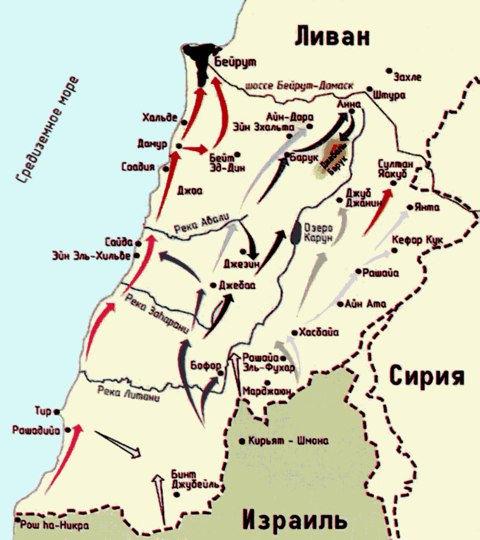
\includegraphics[scale=0.3]{Bekaa_2/v6Lv4fS8Wz4.jpg}
	%	\label{fig:scipion} % Unique label used for referencing the figure in-text\end{document}
	%	%\addcontentsline{toc}{figure}{Figure \ref{fig:placeholder}} % Uncomment to add the figure to the table of contents%----------------------------------------------------------------------------------------
	\caption{Схема израильского наступления}%	CHAPTER 2
\end{figure}

В итоге, до последнего момент не было понятно, как будет развиваться ситуация. Не было понятно, что предпримут сирийцы - в Израиле никто кроме совсем уж отмороженных ястребов не хотел новой большой войны с ними. Предполагалось, что сирийцы сами и под давлением американцев покинут 40-километровую буферную зону, правда их об этом спросить в суматохе как-то забыли.

4-го июня была объявлена тревога по сирийским ВВС, и с того момента сирийские истребители регулярно появлялись над Ливаном - главным образом над северными и центральными районами. На юге действовали израильтяне - и обе стороны до определенного момента стремились не нагнетать обстановку. Долго так продолжаться не могло - и начало боев было вопросом времени, тем более что израильтяне регулярно появлялись в районе Бейрута, и севернее - до поры до времени избегая только долины Бекаа с ее “зонтиком” ПВО..

В ночь на 6-го июня ВВС начали подготовку к наступлению - например, с воздуха были заминированы подходы к Бофору, который планировалось взять силами разведроты бригады Голани на следующий день. Тогда-же ночью вертолеты при поддержке "Скайхоков" атаковали известные артиллерийские позиции, огонь с которых мог помешать продвижению войск. Это были далеко не первые задачи такого рода, на палестинскую артиллерию «Скайхоки» охотились всю предшествующую неделю.

6-го июня после мощного удара авиации по палестинским лагерям “беженцев” и местам сосредоточения террористов, ЦАХАЛ отправился зачищать Ливан. Поначалу все шло неплохо. В гражданской войне, палестинские батальоны неплохо воевали с такими же как они парамилитарными формированиями христиан-маронитов, при встрече с «паровым катком» трёх израильских дивизий их хватило меньше, чем на сутки.

Тогда же ВВС понесли свою первую и единственную потерю в реактивных самолетах — при помощи ПЗРК “Стрела” был сбит “Скайхок” 115-й эскадрильи. Его пилот Аарон Ахиаз, ветеран Войны Судного дня совершил грубейшую ошибку - после неудачного первого захода вместо того, чтобы набрать высоту и скорость и зайти с нового направления на цель, он попытался быстро развернуться и атаковать снова, и в итоге был сбит и попал в плен.

Если у вас вдруг возник вопрос — да, действительно палестинцы сбили больше израильских самолётов, чем вся сирийская армия. Так вышло.

\begin{figure}[h!tb] 
	\centering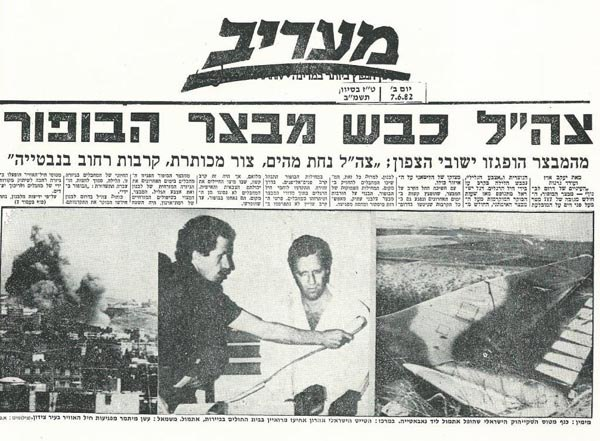
\includegraphics[scale=0.3]{Bekaa_2/LJY5OEnRwx8.jpg}
	%	\label{fig:scipion} % Unique label used for referencing the figure in-text\end{document}
	%	%\addcontentsline{toc}{figure}{Figure \ref{fig:placeholder}} % Uncomment to add the figure to the table of contents%----------------------------------------------------------------------------------------
	\caption{«Доказательство жизни» Аарона Ахиаза}%	CHAPTER 2
\end{figure}

Предполагалось, что сирийцы не будут ввязываться в войну. Однако получилось иначе. Уже на 7-го июня на 2-й день операции произошло первое столкновение в воздухе - над Бейрутом F-15 Офера Лапидота, сына будущего главкома ВВС Амоса Лапидота, второй ракетой (первая “Спэрроу”, как водится, промахнулась) сбил МиГ-23МФ майора сирийских ВВС Али Халляка. Почему? Сириец косо посмотрел радаром в сторону группы “Фантомов”. Сами сирийцы утверждают, что перед этим майор сбил пару F-16, но есть очень большое подозрение, что эти два самолета в тот день вообще не встречались.

Вообще, воздушные бои над Ливаном в тот момент представляли собой достаточно странное зрелище. При всей специфике “арабского” менталитета сирийцы долгое время не испытывали иллюзий относительно исхода прямого столкновения с новыми израильскими истребителями и их старыми пилотами, причем что было для них страшнее - тот еще вопрос. А потому до войны 82 года перед сирийскими летчиками ставилась в первую очередь задача срывать удары израильтян, не вступая в бой на невыгодных для себя условиях. В тот момент, когда израильтяне выводили ударные “Фантомы” и “Скайхоки” в “зону ожидания” над морем, чтобы освободить небо для F-15 и избежать ошибок в идентификации целей - сирийцы уходили в свое воздушное пространство. Часто после этого израильтяне уже не успевали возобновить налет и уходили по остатку топлива. В общем, сирийская тактика действительно какое-то время работала, но долго продолжаться это не могло.

По-сути, сирийские летчики МиГ-21 раз за разом совали голову в пасть льва и с истинно восточным фатализмом рассчитывали на то, что всегда успеют достать ее вовремя. 

\begin{figure}[h!tb] 
	\centering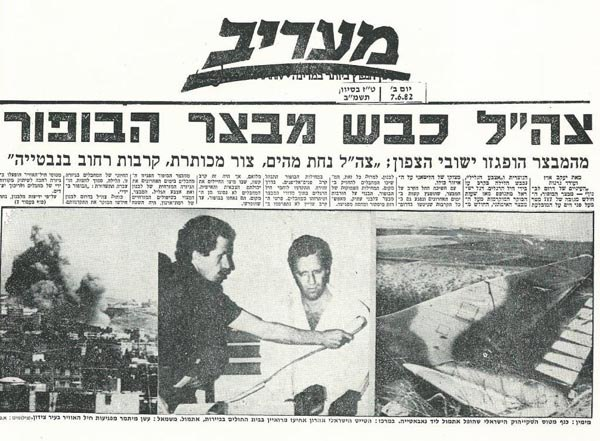
\includegraphics[scale=0.3]{Bekaa_2/LJY5OEnRwx8.jpg}
	%	\label{fig:scipion} % Unique label used for referencing the figure in-text\end{document}
	%	%\addcontentsline{toc}{figure}{Figure \ref{fig:placeholder}} % Uncomment to add the figure to the table of contents%----------------------------------------------------------------------------------------
	\caption{История столкновений 79-82 годов (до 6 июля)}%	CHAPTER 2
\end{figure}

С началом войны у сирийцев не было возможности придерживаться их любимой тактики - израильские налеты были слишком частыми и интенсивными, чтобы тактика “напугай и беги” приносила хоть какой-то результат.

Приходилось сражаться. А тут вырисовывалась проблема - огромный качественный разрыв (и в летчиках, и в самолетах) сводил к нулю возможность вести бой на равных. Точнее — просто вести бой больше пары минут, которые требовались израильтянам для окончательного избиения всего, что летит в их сторону и не несёт бело-голубого опознавательного знака ВВС. А плана "Б" у арабов не было. Точнее, советники из СССР предлагали некоторые идеи, но от "гениальности" многих из них у более адекватных коллег и их сирийских подопечных волосы вставали дыбом.

8-го июня несмотря на все предупреждения израильтян, части сирийской 1-й танковой дивизии начали занимать позиции южнее озера Карун в долине Бекаа для того, чтобы заблокировать израильское наступление в направлении Захле - крупного анклава христиан. Занятая ими территория находилась внутри 40-километровой “буферной зоны”, которую израильтяне планировали занять. В принципе, с этого момента столкновение стало неизбежным.

В этот момент израильское правительство наконец утверждает план “Большие сосны” - только в гораздо худших условиях, чем планировалось изначально, фактически - без фактора внезапности. Теперь достижение его основной цели - шоссе Бейрут - Дамаск - существенно осложнялось.

В общем, 8-го июня на сирийцев обрушились авиация и танки, превосходство в которых у израильтян было колоссальным. Тогда же, 8-го июня, четверка “Дефендеров” выбила сирийскую РЛС в Дамуре (прибрежный город южнее Бейрута), "Фантомы" уничтожили истребительный командный пункт ВВС Сирии под Бейрутом и 2 из 3 основных РЛС, дававших какую-то информацию сирийцам. После этого, сирийцы вообще перестали контролировать всё, что происходит в воздухе западнее Ливанского хребта - то есть всё кроме долины Бекаа. Последнее, как мы понимаем, временно. Вскоре они перестали контролировать вообще что-либо.

Сирийцы бросили в бой ударные МиГ-23БН и “Газели”, первые действовали бестолково и особых проблем не создавали, а вот вторые изрядно нагадили израильским танкистам. Вообще, можно сказать что именно “Газель” была наиболее эффективным сирийским летательным аппаратом всей войны (не считать же таковым советское катапультируемое кресло?) - сказалось подавляющее качественное превосходство новых американских самолётов в воздухе. Уже с первых дней стало понятно, что для ВВС это будет не война, а избиение - 9 лет назад соотношение побед и потерь в воздухе было порядка 1:10 - чего можно было ожидать, когда израильтяне пересядут с “Миражей” и “Фантомов” на F-15 и F-16? Правильно. Сирийцы просто не смогли сбить кого-либо.

Восьмого же июня начались интенсивные совещания насчет того, что с сирийским ракетным щитом в Бекаа надо что-то делать. Он слишком сильно ограничивал поддержку авиации - без нее войска, атаковавшие сирийцев, понесли бы слишком большие потери. К тому-же, под прикрытием ЗРК разворачивались сирийские подвижные соединения.

План атаки батарей к тому моменту был отработан в мельчайших подробностях, все технические средства были многократно протестированы. В общем, ВВС находились в волнительно-радостном предвкушении мести за предыдущую войну.

Изначально, удар по батареям планировался именно 8-го числа. Были назначены летчики, получены боевые задачи, самолеты загружены в наиболее подходящую конфигурацию для борьбы с ПВО. Но решение о начале операции было принято после долгих споров в кабинете Бегина - слишком поздно, чтобы успеть выполнить задачу до конца светового дня. Потому атаку перенесли на один день.

С утра подняли беспилотники, произвели доразведку. “Квадраты” оставались на прежнем месте. В штабе ВВС определили порядок действий и наиболее приоритетные цели. Банк целей пополнился после нескольких разведывательных вылетов БПЛА.

Список задач спустили в эскадрильи.

ВВС были в шаге от того, чтобы войти в историю.

\begin{figure}[h!tb] 
	\centering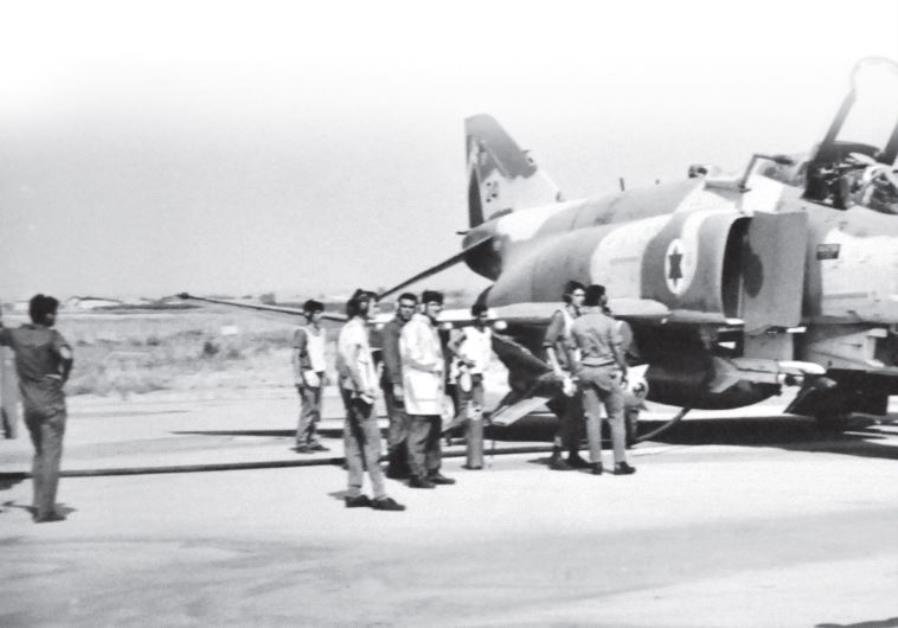
\includegraphics[scale=0.3]{Bekaa_2/58VsCDFGsQY.jpg}
	%	\label{fig:scipion} % Unique label used for referencing the figure in-text\end{document}
	%	%\addcontentsline{toc}{figure}{Figure \ref{fig:placeholder}} % Uncomment to add the figure to the table of contents%----------------------------------------------------------------------------------------
	\caption{201-я эскадрилья "Фантомов" готовится к вылету. Ее комэск Ави Барбер был одним из сбитых во время неудачной операции по подавлению ЗРК в начале Войны Судного дня (Дугман-5) и попал в плен.}
\end{figure}	
	
Итак, "сегодня" - 9 июня 1982 года. На часах - 4 утра. Подходит к концу совещание командования Северного военного округа, с участием начальника Генштаба Рафаэля Эйтана и минобороны Ариэля Шарона. На повестке дня - уничтожение сирийского зонтика ПВО в Бекаа - и полномасштабная война с сирийцами в Ливане. Есть два основных варианта - уничтожить ПВО в Бекаа целиком или ограничиться парой батарей, чтобы создать давление на сирийцев. Принимают первый вариант.

Командование ВВС получает “добро” на атаку. Политики приняли решение - теперь дело за летчиками.

Рано утром несколько беспилотников производят разведку позиций ЗРК в Бекаа. С вечера 8-го июня ничего не изменилось, сирийцы остались на прежних позициях в прежнем составе - 15 дивизионов “Квадратов”, 2 дивизиона С-75М, 2 дивизиона С-125М. Все вместе - три бригады “Квадратов” и одна смешанная. К слову, в Ливане было больше трети ВСЕХ “Квадратов” сирийцев - 15 дивизионов из 41. Кроме этих 15, еще 5 дивизионов было “на подходе” на границе с Ливаном. Но - на сирийской части границы, а потому удар по ним не наносился.

\begin{figure}[h!tb] 
	\centering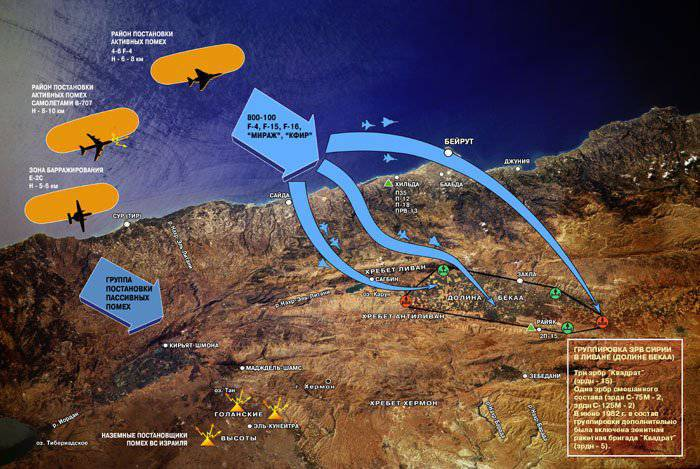
\includegraphics[scale=0.3]{Bekaa_2/9zyt2hCclcQ.jpg}
	%	\label{fig:scipion} % Unique label used for referencing the figure in-text\end{document}
	%	%\addcontentsline{toc}{figure}{Figure \ref{fig:placeholder}} % Uncomment to add the figure to the table of contents%----------------------------------------------------------------------------------------
	\caption{Примерный план операции}
\end{figure}	

Кроме средств ПВО зенитно-ракетных войск, в Бекаа было огромное количество разного рода армейского ПВО - наибольший интерес для израильтян представляли SA-8 (ОСА-АК). Кроме них было порядка 50 “Шилок” и 400 орудий ПВО и расчетов ПЗРК.

Серьезные силы? Безусловно. Если не вникать в детали. Во-первых, при очень высокой плотности боевых порядков, “Феда” была зажата между двумя горными хребтами в прямоугольнике 30 на 28 километров, при отсутствии обзора за ними. То есть фактически сирийцы были у израильтян как на ладони, при этом сами они до последнего момент не могли обнаружить атакующие самолеты. К тому-же, массив Ливанских гор крайне негативно влиял на радиолокацию, и сам по себе отраженный сигнал создавал достаточно неприятные помехи. Во-вторых, радиолокационное обеспечение (то есть поиск и идентификация целей) осуществлялись автономными средствами разведки дивизионов - станции управления и наведения светили во все стороны и излучали как новогодняя ёлка. В-третьих, ЗРК каждой из четырех бригад управлялись с КП этой бригады, причем связи между КП этих самых бригад у сирийцев не было (!). В итоге, каждый воевал сам за себя.

Как только командный пункт бригады, приоритетная цель для израильтян, вскрывался средствами радиотехнической разведки и выводился из строя (а это обычно был лишь вопрос времени, как правило - часа) - батареи ЗРК оставались предоставлены сами себе. В общем, бестолково организованное боевое управление и отсутствие хоть какого-то сопряжения ЗРК КРАЙНЕ СУЩЕСТВЕННО снижало потенциал всей группы.

Часто пишут, что операция началась в 14:00. Это не совсем точно. На 14:00 назначили собственно атаку - а подготовка к ней началась существенно раньше - можно даже сказать, что операция началась 8-го июня, когда вертолеты уничтожили 2 РЛС П-15 в Дамуре. Кстати, про время. Одной из причин выбора времени можно назвать положение солнца - оно как-раз находилось в зените. С учетом того, что в 82-м году израильские ударники как правило работали из глубокого пикирования со средних высот, это было осмысленно. До начала атаки свои позиции заняли самолеты обеспечения - 707 “Боинги”, переделанные в самолеты постановки помех и радиотехнической разведки заняли позицию над Средиземным морем на траверзе Бейрута. Вскоре к ним присоединились взлетевшие из аэропорта Лод самолеты ДРЛО E-2 “Хокай” и “Аравы” - израильские военно-транспортные самолеты, переделанные в постановщики помех. Этим самолетам предстояло сыграть едва ли не ключевую роль в надвигающихся событиях.

На авиабазах, радарных станциях, станциях постановки помех на Голанах, командных пунктах кипела работа. План был следующий:

Приблизительно в 13:30 стартует первая группа “Скайхоков”. Эти машины были практически невооруженными и несли по паре “Шимшонов” - летающих ложных целей, создающих на экране радара отметку полноценного самолета. У запуска ложных целей было две основных задачи. Главная - заставить сирийцев потратить ракеты, чтобы к моменту появления израильских самолетов большая часть пусковых перезаряжалась и не была готова к пуску. Второстепенная - заставить станции управления и наведения батарей “Квадратов” излучать - для того, чтобы выпустить по ним огромное количество противорадарных ракет. В тот момент, когда “Шимшоны” стартовали, в воздухе уже была вторая волна самолетов, в основном “Фантомов”.

Приблизительно в 14:05 под воздействием мощнейших помех, генерируемых самолетами, вертолетами и наземными станциями на Голанах, большинство сирийских станций наведения ЗРК и сирийских РЛС оказались ослепленными. Радиолокационные станции сантиметрового и дециметрового диапазонов были подавлены вкруговую, а для РЛС метрового диапазона секторы эффективного подавления составляли 45-50 градусов - этого было достаточно.

Последнее, что увидели сирийцы перед тем, как их РЛС были забиты помехами — огромное количество целей, идущих с востока. Первые батареи даже успели отстреляться. А потом — они ослепли.

В итоге, радиолокационное поле над Бекаа временно перестало существовать - отдельные станции в глубине боевых порядков еще могли осуществлять проводку целей, но обмен информацией у сирийцев был поставлен крайне плохо. С момента обнаружения цели до момента поступления информации на наземный КП могло пройти 5-10 минут, как правило к тому моменту такая информация становилась немного неактуальной - в тот момент израильтяне уже успевали отбомбиться и были на пути домой. Нередко — сам командный пункт к тому моменту уже переставал существовать.

Имевшиеся на руках у сирийцев средства были просто не в состоянии “держать удар” помех такой мощности - если авиационные средства РЭП еще худо-бедно можно было “переварить”, то наземные станции на Голанах были просто ультимативным оружием.

В тот момент, когда сирийские РЛС и СУРН батарей ЗРК были подавлены помехами, к ним уже летела вторая волна израильских ударных самолетов, в основном “Фантомов” 107-й и 201-й эскадрилий. Они несли два основных типа вооружения - противорадарные ракеты AGM-78 «Стандард-АРМ» (они же “Эргоф Саголь” или Purple fist) и управляемые бомбы AGM-62 “Walleye” (возможно GBU-8 HOBOS). И те и другие - существенно доработанные в Израиле. Первые были выпущены приблизительно с 32 километров, вторые - где-то с 28 из расчета 4 бомбы на батарею. С учетом того, что каждая бомба с учетом доработок стоила астрономический по тем временам миллион долларов - получалось очень недешево. Кроме них, израильтяне использовали “локальную” фишку - ПРР наземного базирования “Кахлилит” и “Керес” - по-сути те - же “Шрайки” и “Стандарты” c телевизионной ГСН, переделанные под наземную ПУ. С “Кахлилитами” вообще получилось забавно - по-сути к “Шрайку” добавили “первую ступень” для увеличения дальности и поставили на шасси старого-доброго Шермана, которых в Израиле было навалом. В общем, голь на выдумки хитра.

С «Эргоф Саголь» (в девичестве AGM-78) связана достаточно забавная история. Американцы предлагали евреям купить их вместе с носителями, специализированными для борьбы с ЗРК F-105G или «Фантомами», «Дикими ласками». Денег на всё это удовольствие в Израиле не нашли, и купили только ракеты, доработав их таким образом, чтобы применять их стало возможно с обычных «Фантомов». Цена боеприпаса выросла в несколько раз, но это всё ещё было дешевле, чем покупать специализированный самолёт.

К авиационным боеприпасам добавляются корректируемые артеллерийские, которыми выбивают дивизионы, находящиеся южнее, ближе к Голанам. Сказывается КРАЙНЕ специфический ТВД - в Европе такое, скорее всего, не прокатило бы.

Во время налета случилось несколько достаточно смешных эпизодов - например, один из “Фантомов” 201-й эскадрильи, внезапно обнаружив перед собой пусковую “Квадрата” и не успевая применить управляемое оружие, использовал пушку - вроде бы как успешно. Не всё шло гладко — отдельные батареи поражались несколько раз, по другим израильтяне не отработали из-за отказов оборудования или общей неразберихи, но сирийцам это мало помогло.

Целеуказание для них давали беспилотники, в количестве висевшие над Бекаа. Их важность сирийцы и советники поняли только после войны - почти сразу поступила команда уничтожать любые подобные цели. 

\begin{figure}[h!tb] 
	\centering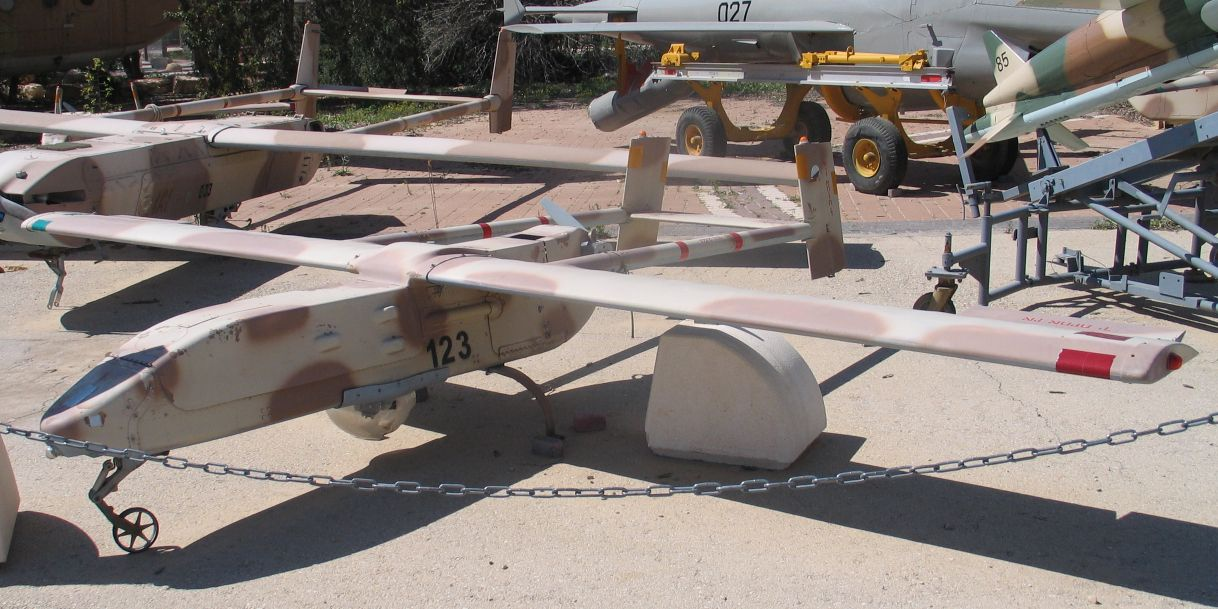
\includegraphics[scale=0.3]{Bekaa_2/Q1AcDv3Bxdc.jpg}
	%	\label{fig:scipion} % Unique label used for referencing the figure in-text\end{document}
	%	%\addcontentsline{toc}{figure}{Figure \ref{fig:placeholder}} % Uncomment to add the figure to the table of contents%----------------------------------------------------------------------------------------
	\caption{БПЛА «Скаут», музей ВВС Израиля в Хацерим}
\end{figure}	

Сирийские расчеты были в панике - они не понимали, как и откуда к ним прилетают ракеты, тем более - с такой удивительной точностью - советники как-то писали (со слов сирийцев), что израильтяне ухитрялись попадать не просто в отдельно стоящую технику, а в открытые люки.
Приблизительно в 14:10-14:20 централизованное управление группой ПВО “Феда” было утрачено вместе с большей частью самой группы. Ослепленные дивизионы добивали кассетными бомбами и боеприпасами объемного взрыва “Скайхоки”, “Фантомы”, “Кфиры” и F-16. Задачей израильтян было именно физически уничтожить всё - пусковые, СУРН, командные пункты дивизионов и бригад. В этот момент можно смело сказать, что из SEAD (подавление ПВО) операция превратилась в DEAD (уничтожение ПВО). В это время сирийцы начали понимать, что что-то идет не так. После победных реляций первых минут связь прервалась. С командных пунктов бригад судорожно пытались достучаться до КП дивизионов и батарей. Безуспешно. Скоро не стало и самих КП бригад. Началась паника. Некоторые командиры дивизионов, четко осознавая, что происходит выключили радары и попытались спрятаться, некоторые из них уцелели. Некоторые попытались перейти на оптический канал наведения - безуспешно. Некоторые пытались вести "заградительный" огонь путём пуска ракет «куда-то вверх» - их останки нашли в конце дня.

Приблизительно в 14:15 сирийцы поднимают первые самолеты - ранее сознательно выведенные из воздушного пространства над Бекаа во избежание дружественного огня. Сирийское командование судорожно кидает все имеющиеся в наличии силы для спасения “Феды”. Сирийцы вступают в бой сразу, по мере взлета, как правило - парами, с достаточно фантасмагорической задачей - “прикрытие ЗРК путем дежурства в воздухе”. Блин, с тем же эффектом можно дежурить в бассейне с акулами. В этот момент “Арцав-19” приостанавливается - имеющиеся ударные самолётыуводят или назад на аэродромы, или в зону ожидания над Средиземным морем. Место ударников занимают F-15 и F-16, барражирующие в слепой для сирийцев зоне между горными хребтами. Начинается бойня - израильтяне спокойно наводят на полуслепые пары МиГ-21 и МиГ-23 перехватчики и последовательно их сбивают. Не то, чтобы всех - но 20-30% потерь за вылет - это уже близко к катастрофе. Часто высокую эффективность израильских истребителей объясняют использованием самолетов ДРЛО “Хокай”. Это отчасти верно, хотя их часто переоценивают - на фоне подстилающей поверхности, особенно гор, они были весьма умеренно эффективны.

Приблизительно в 14:50 сирийцы заканчивают отправлять самолеты. Те из ударников 3-й группы, у которых оставалось достаточно топлива (в основном это были “Скайхоки”) - отправляются в Бекаа. Внезапно большинство из них узнает, что первоначальные полученные им цели больше не актуальны - потому что перестали существовать. “Скайхоки”, “Кфиры” и F-16 направляют атаковать позиции ствольной ПВО, танковых дивизий, колонны снабжения. Ударные самолеты заходят с 2 направлений - со стороны Голан и Средиземного моря.

Вообще, здесь наилучшим образом показали себя “Скайхоки”. Они имели одно ключевое преимущество - возможность висеть в воздухе достаточно долго, в отличие от “Кфиров”, особенно - летавших из Эйлата. С последними была проблема - топлива у них едва-едва хватало на полет до цели, обратно и пару заходов.

“Скайхоки” же могли висеть над целью до часа - бесценное качество, особенно во второй половине операции, когда всякое планирование было бессмысленно. Эти машины составляли треть ударной мощи Израиля. Хотя непосредственно в атаках на ЗРК они практически не принимали участие, но их роль в обеспечении действий “Фантомов” переоценить сложно - это постановка помех, запуск летающих мишеней, удары по батареям ствольной ЗА, и так далее …

Нельзя сказать, что это было просто - сирийцы стреляли из всего, что могли стрелять. Летавшие в Бекаа описывают, что вся долина была затянута практически пеленой, морем зенитного огня. Как только они начинали заходить на цель - огонь становился ураганным. По-этому работать приходилось со средних высот и из пикирования - попытка спуститься ниже неизбежно привела бы к потерям самолетов. Будь ЗРК в порядке - у израильтян были бы проблемы. Но «Квадраты» в Бекаа к тому моменту практически перестали существовать.

К 17:00 операция завершается, последние самолеты возвращаются домой. Дело сделано. Из 19 дивизионов ЗРК уничтожено 15, еще 4 вышло из строя. “Феда” перестала существовать. Еще порядка 18-22 сирийских самолетов сбито над Бекаа (+5-7 утром). Сирийцы деморализованы и паникуют. План “Б” на случай массированного удара по батареям у них отсутствовал - и они, и советники по какой-то причине продолжали жить в 73-м году.

Успех операции предопределило сочетание новых технических средств (зачастую - американских, существенно доработанных “напильником”) и новых тактик - средства РЭП, “Маверики”, “Хобосы” и “Хокаи” у американцев были, а вот возможности управлять авиацией “в реальном времени”, перераспределять звенья по дороге к цели - ещё нет. Для Америки комэск F-15, занимающийся в воздухе обработкой сообщений от “Хокая” и самостоятельно распределяющий задачи для себя и братских эскадрилий - нонсенс. Для израильтян это стало нормой жизни.

Итак, “Феда” пала. Сирийцы отправились зализывать раны - и думать, что в сложившейся ситуации делать. Надежды на новый “зонтик ПВО” не было - было очевидно, что израильтяне размолотят любое ПВО вне зависимости от его состава. Правда, 5 дивизионов “Квадратов” в Бекаа все-же ввели - “Фантомы” добили их утром следующего дня тем же способом, что и в предыдущий день - спровоцировали на излучение - подавили - выбили радары - добили кассетными бомбами. После этого сирийцы вывели уцелевшие комплексы из Ливана и больше не рисковали ими.

В следующей, заключительной части мы поговорим про истребительную авиацию, и выводы, которые сделали из всей этой истории в разных странах.

Ссылка на оригинал \url{https://vk.com/wall-162479647_24373}

К оглавлению на странице \pageref{tablecont}